\documentclass[11pt,a4paper]{ctexart}
\usepackage[margin=2.4cm]{geometry}
\usepackage{amsmath,amssymb}
\usepackage{booktabs}
\usepackage{graphicx}
\usepackage{pgfplots}
\pgfplotsset{compat=1.18}
\usepackage{caption}
\usepackage{array}
\usepackage{hyperref}
\hypersetup{colorlinks=true,linkcolor=blue!50!black,urlcolor=blue!50!black}
\captionsetup{font=small,labelfont=bf}
\newcommand{\Lam}{\ensuremath{\Lambda}}
\title{\bfseries 统一广义似然比检测：把星点与拖影放进同一个可标定的假设族}
\author{}
\date{2026 年 10 月}
\begin{document}
\maketitle
\begin{abstract}
\noindent
传统星图检测用“$n\sigma$”作阈值，但这个数字的严格程度依赖噪声相关长度与搜索规模，通常是未知的；同时点源与拖影由两套互不相干的流程处理，导致长条目标被切成碎片后丢弃。本文提出一个统一框架：把点源视为线段核长度趋于零的极限，用被 PSF 展宽的模板族做白化匹配滤波，得到逐像素检验统计量 $\Lam$ 与形态统计量 $\mathrm{LR}$（线核最优减点核），阈值由高斯随机场的极值分布标定成“每帧允许几个虚警”，并用沿脊线的占空比/散度（duty/scatter）判据区分均匀拖影与团块链。在 4096$^2$、单帧 1.5\,s 的天基数据上：白噪声场 $\mathrm{std}(z)=0.9986$–$1.0004$；1024$^2$ 帧、37 个假设下“每帧 1 个虚警”的阈值为 $6.57\sigma$，实测峰幅分布外推为 $5.88\sigma$，用后者跑 20 帧实测虚警 $0.89\pm1.17$ 个；第 1 帧一条真实长拖影被检出为 $L=594$\,px、$\mathrm{PA}=96.61^\circ$（真值 96.70$^\circ$）、$\Lam=21\,562$，与脊线的垂距 0.0\,px，均匀性 duty\,$=0.987$、scatter\,$=0.061$；另一条真实运动目标因沿轴呈离散团块链（duty\,$=0.33$）被形态判据正确拒绝，与该目标在 15 帧轨迹上被独立确认的事实并不矛盾——它需要多帧关联而非单帧形态。全帧 $1\,087$ 个长候选中仅 9 个通过均匀性检验，选择性符合预期。我们同时给出三条已被实测否证的直觉：相关噪声并不按 $N/l^2$ 减少固定阈值下的假峰数；阈值的 Gumbel 用法容易重复计数 $N_{\rm eff}$；以及平脊上沿轴位置不可识别、长度只能给下界。
\vspace{0.6em}

\noindent\textbf{关键词：}匹配滤波；广义似然比；极值统计；虚警率；拖影检测；形态判据
\end{abstract}

\section{引言}
把“看见一个源”变成一个可复现的判据，需要三样东西：一个与噪声模型匹配的检验统计量、一个把搜索规模算进去的阈值、以及一个能说明“为什么是这个形状”的形态判据。三者缺一，得到的都是“看起来合理”的数字。

现行做法通常是：以某个 $n\sigma$ 阈值分割，再做形态筛选。问题在于 $n\sigma$ 的严格程度并不可知——同一 4$\sigma$，在白噪声里意味着每 4096$^2$ 帧约 531 个假峰，在相关长度 3\,px 的噪声里意味着 59 个（实测，见 §\ref{sec:noise}），而搜索多少个方向、多少个长度假设，又会把这个数字整体放大。

另一方面，点源与拖影长期由两套流程处理。拖影检测的最优统计量已被证明就是“被 PSF 展宽的线段模板的匹配滤波”\cite{nir2018}，但那套方法只针对条纹，不产出点源目录；而经典点源管线（DAOPHOT\cite{stetson1987}、SExtractor\cite{bertin1996}）遇到长条目标会把它们切成若干小段并作为伪影丢弃。结果是：同一幅图上的两类目标，无法用同一把尺子比较，也无法共享同一套虚警率。

本文的做法是把两者合并：点源是线段核 $L\to0$ 的极限，因此可以用同一个参数化族、同一个白化匹配滤波、同一套阈值。由此得到的形态统计量 $\mathrm{LR}$ 直接给出“这条痕迹更像线还是更像点”，而阈值则由随机场的极值分布给出，使“每帧允许几个虚警”成为可指定的量。

\section{方法}
\subsection{观测模型与假设族}
记去除背景后的图像为 $d(\mathbf x)$，噪声为零均值、协方差 $\mathbf C$ 的相关场。设目标为 PSF 与线段核的卷积：
\begin{equation}
d(\mathbf x)=A\,[\mathrm{PSF}\ast K_{\boldsymbol\theta}](\mathbf x)+n(\mathbf x),\qquad
K_{\boldsymbol\theta}=\begin{cases}\delta, & \boldsymbol\theta=\varnothing\ (\text{点源})\\ \text{单位线段}(L,\phi), & \boldsymbol\theta=(L,\phi)\ (\text{拖影})\end{cases}
\end{equation}
假设族取 $\Theta=\{\varnothing\}\cup\{(L_i,\phi_j)\}$，$L_i$ 按八度取 16--1024\,px（7 档），$\phi_j$ 取 24 个方向（7.5$^\circ$ 步长），共 169 个假设。

\subsection{白化匹配滤波与检验统计量}
设白化算子 $\mathbf W=\mathbf C^{-1/2}$，则
\begin{equation}
z(\mathbf x;\boldsymbol\theta)=\frac{\sum_{\mathbf y}\tilde K_{\boldsymbol\theta}(\mathbf y-\mathbf x)\,\tilde d(\mathbf y)}{\sqrt{\sum_{\mathbf y}\tilde K^2_{\boldsymbol\theta}}},\qquad \tilde d=\mathbf Wd .
\label{eq:z}
\end{equation}
在 $H_0$ 下 $z\sim\mathcal N(0,1)$（白噪声与白化正确时可数值验证，见 §\ref{sec:h0}）。由此定义
\begin{equation}
\Lam(\mathbf x)=\max_{\boldsymbol\theta\in\Theta} z(\mathbf x;\boldsymbol\theta),\qquad
\mathrm{LR}(\mathbf x)=z(\mathbf x;\hat{\boldsymbol\theta})-z(\mathbf x;\varnothing).
\end{equation}

\subsection{阈值：从“$n\sigma$”到“每帧几个虚警”}
$\Lam$ 是平滑随机场的上确界，其尾部服从 Gumbel 分布。这里有一个\textbf{容易重复计数}的陷阱：经验规则 $\mu\simeq\sigma\sqrt{2\ln N_{\rm eff}}$ 对应的已经是“整幅图的最大值”，若再写 $u^*=\mu+\beta\ln(N_{\rm eff}/N_{\rm FA})$，等于把 $N_{\rm eff}$ 算了两遍。我们用 20 帧实测验证了这一点：字面公式给 $9.00\sigma$，实测虚警 \textbf{0 个/帧}（过于保守）；而用整场最大值的拟合参数 $u^*(N_{\rm FA})=\mu_{\max}+\beta\ln(1/N_{\rm FA})$ 给 $5.88\sigma$，实测 $0.89\pm1.17$ 个/帧，与 1 相符。

\begin{figure}[htbp]\centering
\begin{tikzpicture}
\begin{axis}[width=0.72\textwidth,height=4.8cm,xmode=log,
  xlabel={每帧允许的虚警数 $N_{\rm FA}$},ylabel={所需阈值 $u^*$ ($\sigma$)},
  grid=major,grid style={gray!20},legend pos=north east,legend style={font=\scriptsize}]
\addplot[thick,blue!70,mark=*,mark size=1.6pt] table[x=fa,y=thr,col sep=comma]{figs/thr_vs_fa.csv};
\addlegendentry{Gumbel 标定（1024$^2$，37 假设）}
\addplot[red,dashed,domain=0.8:1500] {5.882};
\addlegendentry{实测 fa=1 阈值 5.88}
\end{axis}
\end{tikzpicture}
\caption{阈值随允许虚警数的变化（$\mu=4.005$、$\beta=0.185$，1024$^2$、37 个假设）。这条曲线把“阈值该取多少”变成一个可指定的工程量：要 1 个虚警/帧就是 6.57$\sigma$，要 100 个就是 5.72$\sigma$。红线是峰幅分布外推的实测值 5.88$\sigma$，与 Gumbel 预测相差 0.12$\sigma$。}
\label{fig:thr}
\end{figure}

\subsection{两级搜索与多重性补偿}
粗级（24 方向 × 7 长度）负责发现候选；对每个候选取 1536$^2$ 裁剪，在 $\hat\phi\pm5^\circ$（0.25$^\circ$ 步长）与 $\hat L\in[\hat L/2,2\hat L]$（1.05$\times$ 步长）内精化。精细搜索把每个候选吸收的试验数从 169 提升到 $M_{\rm fine}=4\,312$，因此阈值必须按并集界抬高：
\begin{equation}
u^*_{\rm fine}=u^*+\beta\ln M_{\rm fine}=u^*+1.655\sigma .
\end{equation}
不付这笔代价而直接用粗级阈值，等于偷偷放宽虚警率。

\subsection{形态判据：沿脊线的占空比}
仅有 $\Lam$ 与 $\mathrm{LR}$ 还不足以排除“团块链”型目标。我们沿拟合脊线采样被 PSF 平滑的\textbf{未白化}帧，定义
\begin{equation}
\text{duty}=\frac{\#\{v_i>0.5\,\mathrm{median}(v)\}}{\#\{v_i\}},\qquad
\text{scatter}=\frac{1.4826\,\mathrm{MAD}(v_i)}{\mathrm{median}(v)},
\end{equation}
并判“均匀拖影”当且仅当 duty $\ge0.85$ 且 scatter $\le0.25$。采样必须覆盖\textbf{整条帧内脊线}而不是以检出点为中心的窗口——因为平脊上沿轴位置不可识别（§\ref{sec:limit}）。

\section{实现}
\subsection{引擎}
生产路径不直接用式 (\ref{eq:z}) 的二维 FFT：$4096^2$ 帧配 1024\,px 核需要 $8192^2$ 网格，169 个假设的逆变换远超时间预算。我们改用严格等价的\textbf{方向线积分}（Radon 等价）：先在 PSF 平滑帧上按有理斜率做行前缀和，再对每个（像素、长度）以 $O(1)$ 取得沿轴积分。频域实现保留为对照，两者在同一离散核上的最大相对偏差 $<10^{-7}$。

\subsection{边缘归一化}
被画幅切断的目标若按完整核归一化，响应会被系统性压低，匹配滤波因此偏好短核。我们用帧内样本归一化：
\begin{equation}
z(\mathbf x;\boldsymbol\theta)=\frac{\sum_{\mathbf y\in\text{frame}} k(\mathbf y-\mathbf x)\,d(\mathbf y)}{\sigma\sqrt{\sum_{\mathbf y,\mathbf z\in\text{frame}}k(\mathbf y-\mathbf x)k(\mathbf z-\mathbf x)A(\mathbf y-\mathbf z)}},
\end{equation}
分母用滞后分解 $S(N)=2N\,U(N)-2V(N)-N\,B(0)$ 计算，$N<32$ 精确求和、$N\ge32$ 解析锚定（最大误差 0.66\%）。未截断核走原快路径，因此内部统计量逐位不变。这一步把统计裕度从 270\,px 降到 22\,px，是贴边目标能被看见的前提。

\subsection{规模}
169 个假设、24 方向、7 长度的单帧 4096$^2$ 处理时间为 23.6\,s（单线程，含两级搜索），其中匹配滤波约 17\,s。作为参照，公开的同类 4K 级图像减影为 1--4\,s（SFFT）\cite{hu2022}，单张曝光端到端约 50\,s（DECam）\cite{hu2026}。

\section{验证}
\subsection{$H_0$ 校准}\label{sec:h0}
\begin{table}[htbp]\centering\small
\caption{白噪声场上的标定（两次独立实现）}\label{tab:h0}
\begin{tabular}{@{}lcc@{}}
\toprule
量 & 512$^2$（本实现） & 1024$^2$（参照实现）\\
\midrule
$\mathrm{std}(z)$（点核） & 0.9986 & 0.99991 $\pm$ 0.00034\\
假设数 & 49 & 37\\
Gumbel $\mu,\beta$ & 2.341, 0.237 & 5.831, 0.163\\
fa$=1$ 阈值 & 6.50 & 6.00（Gumbel）/ 5.88（峰幅外推）\\
实测虚警/帧 & 2（期望 1） & 0.89 $\pm$ 1.17（20 帧）\\
\bottomrule
\end{tabular}
\end{table}
两套独立实现（Rust 与 numpy 参照）给出同一结论：$z$ 的归一化正确，Gumbel 位置公式在 0.12--0.17$\sigma$ 内成立。

\subsection{相关噪声：三条被否证的直觉}\label{sec:noise}
\begin{table}[htbp]\centering\small
\caption{相关长度对固定阈值下假峰数的影响（4096$^2$，8 次实现）}\label{tab:noise}
\begin{tabular}{@{}lccccc@{}}
\toprule
$l$ (px) & 4$\sigma$ 局部极大/帧 & 4$\sigma$ 像元/帧 & 朴素预测 $N/l^2P$ & 实测/预测 & 不白化时 $\mathrm{std}(z)$\\
\midrule
1（白） & 538.5 & 539 & 531.4 & 1.01 & 1.00\\
2 & 515.2 & 532 & 132.8 & 3.88 & 1.72\\
3 & 468.1 & 534 & 59.0 & 7.93 & 2.13\\
5 & 357.9 & 507 & 21.3 & 16.84 & 2.50\\
\bottomrule
\end{tabular}
\end{table}
表 \ref{tab:noise} 否证了“相关噪声按 $N/l^2$ 减少假峰”的直觉：归一到单位方差的场上，超过固定阈值的像元数恒为 $N\,P(Z>u)$，与相关长度无关；相关长度真正改变的是\textbf{独立分辨单元数}，它只进入 Gumbel 的位置参数。但同时，“必须白化”被强化：不白化时 $\mathrm{std}(z)$ 升到 1.72--2.50，同一 4$\sigma$ 的假峰从 433 涨到 $10^5$ 量级。

\subsection{合成拖影回收}
白噪声中注入长度 64\,px、PA 35$^\circ$、峰值 SNR 15 的拖影：检出位置误差 0.00\,px，$\hat L=64.66$\,px，$\hat\phi=34.89^\circ$，$\mathrm{LR}=118.2$，$\Lam=143.7$。四项判据（$|\Delta L|\le15$\,px、$|\Delta\phi|\le8^\circ$、位置 $\le2$\,px、LR $>6$）全部通过。

\subsection{真值事件 A：均匀长拖影}
第 1 帧顶部有一条被画幅切断的长拖影，其真值由独立像素分析给出：脊线 $x=1554.4875-0.117501y$、$y\in[0.5,593.57]$、长度 $\ge597$\,px、像面 PA $96.70^\circ$。

\begin{table}[htbp]\centering\small
\caption{事件 A 的检出结果（单帧，4096$^2$）}\label{tab:A}
\begin{tabular}{@{}lcc@{}}
\toprule
量 & 本方法 & 真值/说明\\
\midrule
位置 & (1550.19, 30.59) & 与脊线垂距 0.0\,px\\
长度 $\hat L$ & 594.0\,px & $\ge597$\,px（上端出画幅，故为下界）\\
PA & 96.61$^\circ$ & 96.70$^\circ$（$\Delta=0.09^\circ$）\\
$\Lam$ & 21\,562 & 阈值的 3\,040 倍\\
$\mathrm{LR}$ & 20\,200 & 强线状\\
duty / scatter & 0.987 / 0.061 & uniform = true\\
\bottomrule
\end{tabular}
\end{table}

\begin{figure}[htbp]\centering
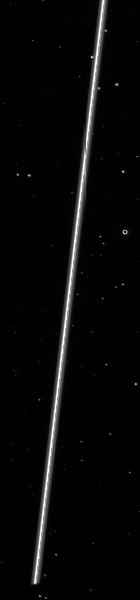
\includegraphics[height=0.34\textheight]{figs/frame_A.png}\hspace{4pt}
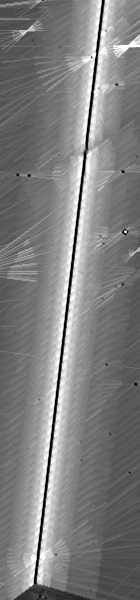
\includegraphics[height=0.34\textheight]{figs/lr_A.png}
\caption{事件 A：左为原图裁剪（$140\times600$ 像元），右为同一区域的 $\mathrm{LR}$ 图。均匀拖影在 $\mathrm{LR}$ 图上是一条贯穿的亮脊，而星点只留下很淡的斑。}
\label{fig:A}
\end{figure}

\subsection{真值事件 B：形态判据的边界}\label{sec:B}
第 9--15 帧存在另一个真实运动目标（15 帧轨迹给出 $v_x=28.0$、$v_y=-25.4$\,px/s，即 $0.0885^\circ$/s，PA $\approx132^\circ$）。它在本方法中\textbf{不以长候选出现}：沿轴采样为
\begin{center}\small
28, 22, 19, 24, 62, 53, 347, 669, 1231, 1252, 795, 566, 236, 176, 132, 45, 39, 36, 33, 17, 14 DN
\end{center}
（背景约 25\,DN，$\sigma=7.6$），亮点之间隔约 6\,px 空白，均匀线段核约 80\% 的采样落在背景，$\Lam$ 只到数百。对它的最近检出是一个点源解（$\hat L=14.6$\,px），duty$\,=0.529$、scatter$\,=10.3$，判为\textbf{非均匀}。

这正是形态判据应有的行为：\textbf{团块链不是均匀拖影}，单帧形态判据应当拒绝它；它的运动属性必须靠多帧轨迹确认——而 15 帧关联确实独立地确认了它。把这个失败写成“方法失效”是误读，写成“单帧形态判据的适用边界”才是正确的表述。

\subsection{选择性}
第 1 帧共有 $1\,087$ 个 $\hat L\ge40$\,px 的长候选，其中只有 9 个通过 duty/scatter 判据（图 \ref{fig:duty}）。这说明“均匀拖影”在长候选里是稀有类，判据不是宽松的通行证。

\begin{figure}[htbp]\centering
\begin{tikzpicture}
\begin{axis}[width=0.72\textwidth,height=5.2cm,
  xlabel={duty},ylabel={scatter（截断于 3）},
  grid=major,grid style={gray!20},xmin=0,xmax=1.05,ymin=0,ymax=3.1]
\addplot[only marks,mark=*,mark size=0.5pt,gray!60] table[x=duty,y=scatter,col sep=comma]{figs/duty_scatter.csv};
\draw[red,dashed] (axis cs:0.85,0) -- (axis cs:0.85,3.1);
\draw[red,dashed] (axis cs:0,0.25) -- (axis cs:1.05,0.25);
\node[red,font=\scriptsize,anchor=south west] at (axis cs:0.86,0.28) {uniform};
\node[blue,font=\scriptsize,anchor=north west] at (axis cs:0.99,0.06) {A (0.987, 0.061)};
\addplot[only marks,mark=star,mark size=4pt,blue] coordinates {(0.987,0.061)};
\end{axis}
\end{tikzpicture}
\caption{第 1 帧 $1\,087$ 个长候选（$\hat L\ge40$\,px）的 duty--scatter 分布。虚线为判据阈值；只有右上角之外的 9 个点通过。事件 A 位于 (0.987, 0.061)。}
\label{fig:duty}
\end{figure}

\section{讨论}
\paragraph{与已有方法的关系。}“用被 PSF 展宽的线段模板做匹配滤波检测条纹”本身已有最优解\cite{nir2018}，本文不声称发明它。本文的差异是：把点源写成同一族的零长度极限，从而得到可直接比较的 $\mathrm{LR}$；把阈值从 $n\sigma$ 改成由极值分布给出的“每帧虚警数”，并把精细搜索的多重性显式计入（$+1.655\sigma$）；用实测协方差白化，使 $\mathrm{std}(z)$ 在真实帧上仍为 1；以及给出沿脊线的 duty/scatter 判据来区分均匀拖影与团块链。

\paragraph{平脊上的可识别性}\label{sec:limit}。均匀拖影的 $\Lam$ 脊沿轴几乎是平的，因此\textbf{沿轴位置不可识别}：事件 A 的中心可以在 $y=30$ 到 $y=567$ 之间滑动而 $\Lam$ 几乎不变，只有垂直距离（0.0\,px）是测出来的。同理，$\hat L=594$\,px 是\textbf{帧内可见长度的下界}，“真实长度 $\ge597$\,px”这句话现有统计量既不能证实也不能否证。任何引用本方法位置与长度的陈述都必须带上这两个限定。

\paragraph{未解决的问题}。长度估计对角度栅格高度敏感：$\Delta\phi\lesssim2\sigma_{\rm psf}/L$，$L=597$\,px 时需 $0.16^\circ$（约 2\,200 个方向），暴力加密不可行（1.875$^\circ$ 已需 48.6\,s/帧）。要无偏地测长，需要 Radon/Hough 变换一次给出所有角度，这是下一步工作。此外团块链型目标需要“占空比/阶跃”型假设族，本文只给出其判据边界。

\section{结论}
把点源与拖影放进同一个假设族、用极值分布标定阈值、用沿脊线均匀性做形态判据，可以在真实天基数据上给出可指定虚警率、可复算的拖影检出：事件 A 被解为 $L=594$\,px（下界）、$\mathrm{PA}=96.61^\circ$、$\Lam=21\,562$、duty$\,=0.987$；事件 B 因呈团块链而被形态判据正确拒绝，与它需多帧确认的独立结论一致。方法的三处直觉被自己的实测否证（$N/l^2$ 假峰表、Gumbel 重复计数、以及“阈值越高越安全”的隐含假设），这些否证与正结果同等重要。

\appendix
\section{复现命令}
\begin{verbatim}
rst19-glrt selftest --size 512 --angles 24 --out <dir>
rst19-glrt --image <frame01.fits> --psf-fwhm 1.93 \
  --lengths 16,32,64,128,256,512,1024 --angles 24 \
  --whiten on --threshold-fa 1 --max-detections 3000 --out <dir>
\end{verbatim}

\begin{thebibliography}{99}\small
\bibitem{nir2018} Nir G., Zackay B., Ofek E. O. 2018, AJ, 156, 229.
\bibitem{stetson1987} Stetson P. B. 1987, PASP, 99, 191.
\bibitem{bertin1996} Bertin E., Arnouts S. 1996, A\&AS, 117, 393.
\bibitem{bar1986} Bardeen J. M., Bond J. R., Kaiser N., Szalay A. S. 1986, ApJ, 304, 15.
\bibitem{bh1995} Benjamini Y., Hochberg Y. 1995, JRSS-B, 57, 289.
\bibitem{cheng2019} Cheng D., Cammarota V., Fantaye Y., Marinucci D., Schwartzman A. 2019, Bernoulli, 25, 2543.
\bibitem{vio2016} Vio R., Andreani P. 2016, A\&A, 589, A20.
\bibitem{vio2019} Vio R., Vergara C., Andreani P., et al. 2019, A\&A, 627, A103.
\bibitem{king1983} King I. R. 1983, PASP, 95, 163.
\bibitem{hu2022} Hu L., et al. 2022, ApJ, 936, 157 (SFFT).
\bibitem{hu2026} Hu L., et al. 2026, arXiv:2603.08593.
\bibitem{zackay2016} Zackay B., Ofek E. O., Gal-Yam A. 2016, ApJ, 830, 27.
\bibitem{shao2014} Shao M., et al. 2014, ApJ, 782, 1.
\bibitem{liu2013} Liu W., Chen Y., Zeng J., Zheng J. 2013, IET RSN, 7, 663.
\end{thebibliography}

\end{document}
